\section{Pilot Findings}

\subsection{License labels and companion text}

After trimming, lowercasing, and filling blank labels, the repository table held 42 distinct license strings, among them MIT, Apache-2.0, GPL-3.0, and AGPL-3.0.
These strings describe the repository that hosts a skill, so they are a data check rather than an answer about the projects that publish taught tools.
We also classified the 3{,}486{,}179 non-blank texts stored beside a skill, and Table~\ref{tab:companion-kinds} shows that almost all of them are free text or JSON objects.
Both kinds include scripts and configuration, so companion text is not skill prose, and extraction stays on the skill body.

\begin{table}[ht]
  \centering
  \caption{Kinds of non-blank text stored beside a skill.}
  \label{tab:companion-kinds}
  \smallskip
  \begin{tabular}{lrr}
    \toprule
    Kind                    & Rows          & Share (\%) \\
    \midrule
    Free text               & 3{,}236{,}628 & 92.8       \\
    JSON object             & 238{,}834     & 6.9        \\
    JSON array              & 10{,}523      & 0.3        \\
    Other JSON\footnotemark & 194           & 0.0        \\
    \bottomrule
  \end{tabular}
\end{table}
\footnotetext{A JSON value that is a string, a number, a boolean, or null.}

\subsection{Label-only model run}

Before we settled on the skill body, a seeded draw of 500 companion texts, each clipped to its first 384 characters, was passed through the label-only model at a score cutoff of~$0.8$.
Figure~\ref{fig:label-only-top} shows every span found in at least two texts, and no bar comes near 500 because the cutoff drops every lower-scoring span, so many texts return no span at all.
The chart also shows why a human check is needed, since the skill filename is marked as a tool even though it names the document itself, and GitHub, which leads with nine files, can be the site inside an address, the place the skill is published, or an attribution link, while none of these labels has a measured error rate.

\begin{figure}[ht]
  \centering
  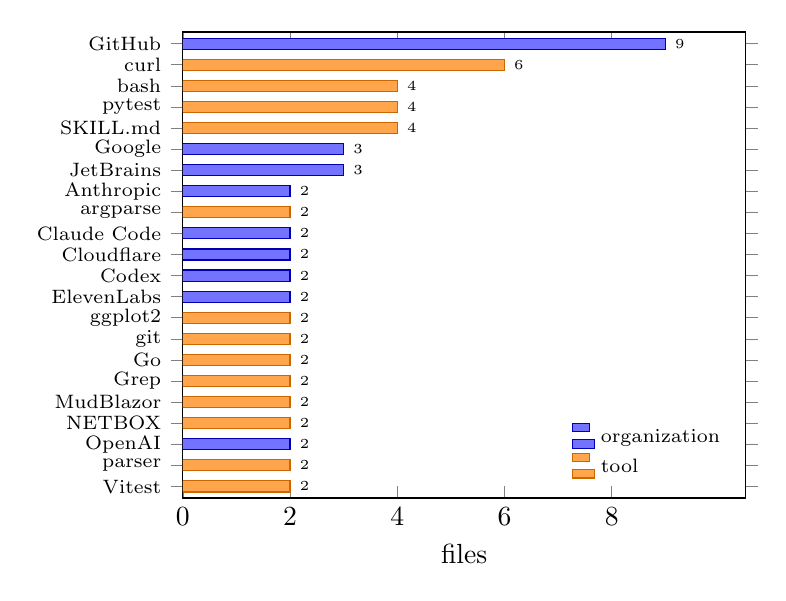
\begin{tikzpicture}
\begin{axis}[
  xbar,
  width=0.72\textwidth,
  height=7.5cm,
  bar width=4pt,
  bar shift=0pt,
  enlarge y limits={abs=0.55},
  xmin=0,
  xmax=10.5,
  xtick={0,2,4,6,8},
  xlabel={files},
  ylabel={},
  ytick={1,...,22},
  yticklabels={
    Vitest,
    parser,
    OpenAI,
    NETBOX,
    MudBlazor,
    Grep,
    Go,
    git,
    ggplot2,
    ElevenLabs,
    Codex,
    Cloudflare,
    Claude Code,
    argparse,
    Anthropic,
    JetBrains,
    Google,
    SKILL.md,
    pytest,
    bash,
    curl,
    GitHub
  },
  yticklabel style={font=\scriptsize, anchor=east},
  nodes near coords,
  every node near coord/.append style={font=\tiny},
  nodes near coords align={horizontal},
  legend style={
    at={(0.98,0.02)},
    anchor=south east,
    font=\scriptsize,
    cells={anchor=west},
    draw=none,
    fill=none
  },
  legend cell align=left,
]
% y=22 is GitHub at the top of the chart.
\addplot[fill=blue!55, draw=blue!70!black] coordinates {
  (9,22)
  (3,17)
  (3,16)
  (2,15)
  (2,13)
  (2,12)
  (2,11)
  (2,10)
  (2,3)
};
\addplot[fill=orange!70, draw=orange!80!black] coordinates {
  (6,21)
  (4,20)
  (4,19)
  (4,18)
  (2,14)
  (2,9)
  (2,8)
  (2,7)
  (2,6)
  (2,5)
  (2,4)
  (2,2)
  (2,1)
};
\legend{organization,tool}
\end{axis}
\end{tikzpicture}

  \caption{Spans that the label-only model found in at least two of 500 companion texts at a score cutoff of 0.8, counted as distinct files after folding case.
    Bars stay small because many texts return no span above the cutoff.}
  \label{fig:label-only-top}
\end{figure}
